% !TEX root = ../slides.tex
\section{Differential cryptanalysis of conjugate ciphers}

{
\setbeamercolor{background canvas}{bg=ptblue}	
\begin{frame}[plain]
\vfill
\begin{center}
%\color{white} \Huge \Roman{section} -  \secname
\color{white} \Huge \secname
\end{center}
\vfill
\end{frame}
}

\subsection{Changing our point of view}
\begin{frame}
\frametitle{\subsecname}
\vspace{-.7cm}
\begin{mybox}{Chosen plaintext access = freedom of study}{}{}
\begin{itemize}
	\item[1)] Encrypt $\blue{H}(x)$ \hspace{1cm}$\leadsto$ $E_{\red{k}} \comp \blue{H} (x)$
	\item[2)] Apply $\changevar$ \hspace{1.88cm}$\leadsto$ $\changevar \comp E_{\red{k}} \comp \blue{H} (x)$
	\item[3)] Study $ \changevar \comp E_{\red{k}} \comp \blue{H} $
\end{itemize}
\end{mybox}

\onslide<2->{
\begin{mybox}{Conjugation}{}{}
The conjugate of $F$ relative to $\changevar$ is the function $\changevar \comp F \comp \changevar^{-1}$ denoted by $F^{\changevar}$.


\vspace{.2cm}
$F^{\changevar}$ is the \emph{same function} as $F$, \emph{up to a change of variables}.
\end{mybox}}
\onslide<3->{
\vspace{-.4cm}
$$ E_{\red{k}} = F_{\red{k^{(R-1)}}} \comp \dotsc \comp F_{\red{k^{(1)}}} \comp F_{\red{k^{(0)}}}$$
}
\onslide<4->{
\vspace{-.2cm}
$$ E_{\red{k}}^{\changevar} = F_{\red{k^{(R-1)}}}^{\changevar} \comp  \dotsc \comp F_{\red{k^{(1)}}}^{\changevar} \comp F_{\red{k^{(0)}}}^{\changevar}$$

Proof left as exercice.\ $\square$ \hfill$(\changevar^{-1} \comp \changevar = \id)$}

% \pause
% \begin{mybox}{Fun fact}{}{}
% For any $ \changevar \from \FFspace \to \FFspace$ bijective, $\changevar^{-1} \comp \changevar = \id$
% \end{mybox}
% \pause
% $$ E_{\red{k}} = \roundF{R-1}_{\red{k}} \comp \changevar^{-1} \comp \changevar \dotsc \comp \changevar^{-1} \comp \changevar \comp \roundF{1}_{\red{k}} \comp \changevar^{-1} \comp \changevar \comp \roundF{0}_{\red{k}}$$
% \pause
% \blue{Conjugate} \& gather terms\hfill \only<5->{$F^{\changevar} \vcentcolon= \changevar \comp F \comp \changevar^{-1}$}
% \only<4>{$$ \blue{G} \comp E_{\red{k}} \comp \blue{G}^{-1} = \left(\blue{G} \comp \roundF{R-1}_{\red{k}} \comp \changevar^{-1} \right) \comp \changevar \dotsc \comp \changevar^{-1} \comp \left(\changevar \comp \roundF{1}_{\red{k}} \comp \changevar^{-1}\right) \comp \left(\changevar \comp \roundF{0}_{\red{k}} \comp \blue{G}^{-1}\right)$$}
% \only<5->{$$ E_{\red{k}}^{\changevar} = \left(\roundF{R-1}_{\red{k}}\right)^{\changevar} \comp  \dotsc \comp \left(\roundF{1}_{\red{k}}\right)^{\changevar} \comp \left(\roundF{0}_{\red{k}}\right)^{\changevar}$$}
\onslide<5>{
\begin{center}
\inlinebox{\large \red{Is it simpler to attack $\black{E}_{\red{k}}^{\changevar}$ than $\black{E}_{\red{k}}$ ?}}
\end{center}}



\end{frame}


\subsection{Linear VS non-linear change of variables}
\begin{frame}
\frametitle{\subsecname}
\vspace{-.4cm}
\begin{recap}
$F^{\changevar} \vcentcolon= \changevar \comp F \comp \changevar^{-1}$
\end{recap}
\vspace{-.4cm}
$$ E_{\red{k}}^{\changevar} = F_{\red{k^{(R-1)}}}^{\changevar} \comp  \dotsc \comp F_{\red{k^{(1)}}}^{\changevar} \comp F_{\red{k^{(0)}}}^{\changevar}$$\pause

\vspace{-.5cm}
\begin{mybox}{Definition/Proposition}{Affine equivalence}{}
    \green{Def}: $F_{1} \aff F_{2}$ if $\quad \exists \ \pcomA, \pcomB$ bijective affine s.t. $\quad \pcomA \comp F_{1} \comp \pcomB = F_{2}$.


    \vspace{.2cm}
    \green{Prop}: If  $F_{1} \aff F_{2}$, then $\delta(F_{1}) = \delta(F_{2})$ and $\linearity(F_{1}) = \linearity(F_{2})$
\end{mybox}
\pause
\begin{corollary}
	$\bulletpoint$ If $\changevar$ linear, $\delta(F) = \delta(F^{\changevar})$ and $\linearity(F) = \linearity(F^{\changevar})$

	\hfill $\implies$ {\small{Fine-grained arguments are needed.}}

	$\bulletpoint$ If $\changevar$ non-linear ?

		\hspace*{7.16cm} $\implies$ {\small{Linear attack cf. \purple{[BeiCanLea18]}}}

		\hfill $\implies$ {\small{Differential attack cf. \purple{[\blue{B}FLNPS23,\blue{B}BFLNPS24]}}}
\end{corollary}

\end{frame}



\subsection{Non-linear change of variables (1/3)}
\begin{frame}
\frametitle{\subsecname}
\vspace{-.7cm}
$$ F_{\red{k^{(i)}}} = T_{\red{k^{(i)}}} \comp \MC \comp \SC \comp \sboxlayer \quad \quad \scalemath{2}{\leadsto} \quad  \quad F_{\red{k^{(i)}}}^{\changevar} = T_{\red{k^{(i)}}}^{\changevar} \comp \MC^{\changevar} \comp \SC^{\changevar} \comp \sboxlayer^{\changevar}$$\pause

\vspace{-.5cm}
\begin{mybox}{Main problem}{}{}
If $F$ is \emph{linear}, $F^{\changevar}$ is a priori not.

$\implies$ $T_{\red{k}}^{\changevar}$ \emph{non-linear dependency} in the key bits.

\end{mybox}
\pause
\vspace{.2cm}
\begin{mybox}{The usual case}{}{}
For all $\plaindiff$ and all $\red{k}$: \ $\proba{\diff[T_{\red{k}}][\plaindiff][\plaindiff]} = 1$

\vspace{.1cm}
$$ T_{\red{k}}(x + \plaindiff) = x + \plaindiff + \red{k} = T_{\red{k}}(x) + \plaindiff$$
\end{mybox}

\pause
\vspace{.1cm}
\begin{mybox}{A possible solution}{}{}
\green{Conjugated case} For \emph{some} $\plaindiff$ and \emph{some} $\red{k}$: \ $\proba{\diff[T_{\red{k}}^{\changevar}][\plaindiff][\plaindiff]} = 1$

\hfill $\implies$ \emph{Weak-key attacks}!
\end{mybox}
% \begin{mybox}{Weak-key space}{}{}
% $W(\plaindiff) = \set{\red{k},\  \proba{\diff[T_{\red{k}}^{\changevar}][\plaindiff][\plaindiff]} = 1} \onslide<5>{ = \set{\red{k},\  \deriv{\plaindiff}T_{\red{k}}^{\changevar} \text{ constant and equal to \plaindiff}} $ 

% \vspace{-.2cm}
% \hfill $\implies$ \emph{linear structure}}
% \end{mybox}

\end{frame}

\subsection{Non-linear change of variables (2/3)}
\begin{frame}
\frametitle{\subsecname}
\vspace{-.7cm}
\begin{recap}
\green{Conjugated case} For \emph{some} $\plaindiff$ and \emph{some} $\red{k}$: \ $\proba{\diff[T_{\red{k}}^{\changevar}][\plaindiff][\plaindiff]} = 1$
\end{recap}

\vspace{-.5cm}
\pause
\begin{mybox}{Weak-key space}{}{}
$W(\plaindiff) = \set{\red{k},\  \proba{\diff[T_{\red{k}}^{\changevar}][\plaindiff][\plaindiff]} = 1}$
\end{mybox}

$$\proba{\diff[T_{\red{k}}^{\changevar}][\plaindiff][\plaindiff]} = 1 \quad \iff \quad \forall \ x, T_{\red{k}}^{\changevar}(x) + T_{\red{k}}^{\changevar}(x + \plaindiff) = \plaindiff $$

\pause
\begin{definition}[Derivative]
The function $\deriv{\plaindiff}F \from x \mapsto F(x) + F(x + \plaindiff)$ is the \emph{derivative} of $F$ along the direction $\plaindiff$.
\end{definition}

\pause
$$\proba{\diff[T_{\red{k}}^{\changevar}][\plaindiff][\plaindiff]} = 1 \quad \iff \quad \deriv{\plaindiff}T_{\red{k}}^{\changevar} \text{ is constant}$$

\end{frame}



\subsection{Non-linear change of variables (3/3)}
\begin{frame}
\frametitle{\subsecname}
\vspace{-.7cm}
\begin{mybox}{Intuition}{}{}
$T_{\red{k}}^{\changevar}$ with constant derivatives $\scalemath{2}{\leadsto}$ $\quad T_{\red{k}}^{\changevar} = \changevar \comp T_{\red{k}} \comp \changevar^{-1}$ somehow close to be linear.
\end{mybox}
\pause
\begin{mybox}{Our explored space}{}{}
$\changevarlayer$ Sbox layer based on $\changevar \from \FF_{2}^{4}\to \FF_{2}^{4}$ with $$\changevar \left(x_{0},~x_{1},~x_{2},~x_{3}\right) = \left(x_{0} + \orange{g}(x_{1}, x_{2}, x_{3}),~x_{1},~x_{2},~x_{3}\right)$$
\hfill ($\changevar = \changevar^{-1}$)

\end{mybox}
\pause
\vspace{-.2cm}
\begin{columns}[c]
\begin{column}{0.3\textwidth}


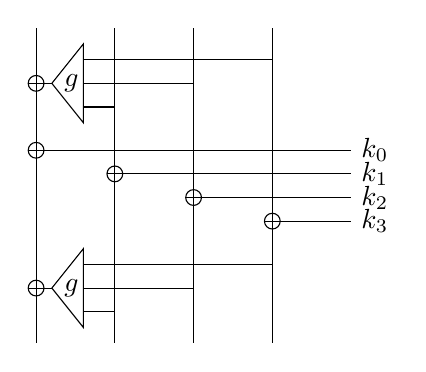
\begin{tikzpicture}

\draw (0, 0) -- +(0, -4);
\draw (1, 0) -- +(0, -4);
\draw (2, 0) -- +(0, -4);
\draw (3, 0) -- +(0, -4);

\draw (-.1, -.7) -- + (.3, 0);
\draw (1, -1) -- + (-.4, 0);
\draw (2, -.7) -- + (-1.4, 0);
\draw (3, -.4) -- + (-2.4, 0);
\draw (0.2, -.7) -- (.6, -1.2) -- (.6, -.2) -- (0.2, -.7);
\node at (.45, -.7) {$\orange{g}$};

\draw (-.1, -1.55) -- + (4.1, 0) node[right=.2] {$\red{k_{0}}$};
\draw (.9, -1.85) -- + (3.1, 0) node[right=.2] {$\red{k_{1}}$};
\draw (1.9, -2.15) -- + (2.1, 0) node[right=.2] {$\red{k_{2}}$};
\draw (2.9, -2.45) -- + (1.1, 0) node[right=.2] {$\red{k_{3}}$};
\draw (0,-1.55) circle (.1);
\draw (1,-1.85) circle (.1);
\draw (2,-2.15) circle (.1);
\draw (3, -2.45) circle (.1);

\draw (-.1, -3.3) -- + (.3, 0);
\draw (1, -3.6) -- + (-.4, 0);
\draw (2, -3.3) -- + (-1.4, 0);
\draw (3, -3) -- + (-2.4, 0);
\draw (0.2, -3.3) -- (.6, -3.8) -- (.6, -2.8) -- (0.2, -3.3);
\node at (.45, -3.3) {$\orange{g}$};

\draw (0,-.7) circle (.1);
\draw (0,-3.3) circle (.1);

\end{tikzpicture}
\end{column}
\begin{column}{0.7\textwidth}
$$T_{\red{k}}^{\changevar} (x_{0},~x_{1},~x_{2},~x_{3}) = \left(\begin{array}{l}x_{0} + \red{k_{0}} + \deriv{\red{\widetilde{k}}}\orange{g}(x_{1},x_{2},x_{3}) \\ x_{1} + \red{k_{1}}\\ x_{2} + \red{k_{2}}\\ x_{3} + \red{k_{3}}\end{array}\right)$$
\vspace{.3cm}
\pause
\begin{center}
$\orange{g}$ quadratic $\implies$ $T_{\red{k}}^{\changevar}$ linear $\implies$ constant derivatives $\deriv{\plaindiff}T_{\red{k}}^{\changevar}$
\end{center}
\end{column}
\end{columns}
\end{frame}

\subsection{The case of Midori}
\begin{frame}
\frametitle{\subsecname}
\vspace{-.4cm}
\begin{mybox}{Sbox}{}{}
By computer search, there exist $\changevar$ and $\plaindiff$ s.t $\proba{\diff[\cyan{S}^{\changevar}][\plaindiff][\plaindiff]} = 1$ \hfill $ \proba{\diff[\scalemath{1.05}{\cyan{\sboxlayer}}^{\changevarlayer}][\bnabla][\bnabla]} = 1$.

$\bnabla = (\plaindiff, \dotsc, \plaindiff)$. 
\end{mybox}
\pause
\begin{mybox}{Linear layer}{}{}
% $\scalemath{.9}{M^{\changevar}_{0} \left(\begin{array}{l}x\\ y\\  z\\  t\end{array}\right) = \left(\begin{array}{l} y_{0} + z_{0} + t_{0} + \orange{g}(y) + \orange{g}(z) + \orange{g}(t) + \orange{g}(y + z + t) \\ y_{1} + z_{1} + t_{1}\\ y_{2} + z_{2} + t_{2}\\ y_{3} + z_{3} + t_{3}\end{array}\right)} \quad \quad
$\scalemath{.9}{M = \left(\begin{array}{cccc} 0 & \id & \id & \id\\ \id & 0 & \id & \id\\ \id & \id & 0 & \id\\ \id & \id & \id & 0
\end{array}\right)}$\hfill $ \proba{\diff[\scalemath{1.05}{\orange{\MC}}^{\changevarlayer}][\bnabla][\bnabla]} = 1$
\end{mybox}
\pause

\begin{mybox}{Probability-1 distinguisher for infinitely many rounds$^{\red{\scalemath{1.1}{\star}}}$}{}{}
$$ \scalemath{.9}{\proba{\bnabla \xrightarrow{\cyan{\sboxlayer}^{\changevarlayer}} \bnabla \xrightarrow{( \orange{MC} \comp \SC )^{\changevarlayer}} \bnabla \xrightarrow{T_{\red{k^{(0)}}}^{\changevarlayer}} \bnabla \xrightarrow{\cyan{\sboxlayer}^{\changevarlayer}} \bnabla \xrightarrow{( \orange{MC} \comp \SC)^{\changevarlayer}} \bnabla \xrightarrow{T_{\red{k^{(1)}}}^{\changevarlayer}} \bnabla \xrightarrow{\cyan{\sboxlayer}^{\changevarlayer}} \bnabla \xrightarrow{(\orange{MC} \comp \SC)^{\changevarlayer}} \bnabla \xrightarrow{T_{\red{k^{(0)}}}^{\changevarlayer}} \cdots}} = 1 $$

\vspace{-.3cm}
$^{\scalemath{1.1}{\red{\star}}}$ If the two round keys are weak. $ \frac{\card{W(\bnabla)}}{2^{64}} = 2^{-16}$\hfill $\implies$ $2^{96}$ weak-keys for \emph{variants} of Midori
\end{mybox}
\end{frame}


\subsection{Equivalent points of view}
\begin{frame}
\frametitle{\subsecname}
\vspace{-.7cm}
\begin{align*}
	\onslide<1->{\PP\big[\diff[F^{\changevar}][\din][\dout] \big] = 1 \quad &\iff \quad \forall \ x, F^{\changevar}(x + \din) + F^{\changevar}(x) = \dout\\}
	\onslide<2->{&\iff \changevar \comp F \comp \changevar^{-1} \comp T_{\din} = T_{\dout} \comp \changevar \comp F \comp \changevar^{-1}\\}
	\onslide<3->{&\iff F \comp \underbrace{(\changevar^{-1} \comp T_{\din} \comp \changevar)}_{\pcomA} =\underbrace{(\changevar^{-1} \comp T_{\dout} \comp \changevar)}_{\pcomB} \comp F}
\end{align*}

\onslide<4->{
\begin{mybox}{Equivalent points of view}{}{}
\begin{itemize}
	\item[\bulletpoint] ``Commutation'' \quad $F \comp \pcomA = \pcomB \comp F$\hfill \purple{\small[\blue{B}FLNPS23]}
	\onslide<5->{\item[\bulletpoint] Self-equivalence \quad $\pcomB^{-1} \comp F \comp \pcomA = F$\hfill \purple{\small[\blue{B}FLNPS23]}}
	\onslide<6->{\item[\bulletpoint] Differential eq. for \emph{another group law} \quad $F \comp (\changevar^{-1} \comp T_{\din} \comp \changevar) =(\changevar^{-1} \comp T_{\dout} \comp \changevar) \comp F$

	$\changevar^{-1} T_{\plaindiff} \changevar$ is an addition, up to a change of variables.\hfill \purple{\small [CivBloSal19, CalCivInv24]}}
\end{itemize}
\end{mybox}}

% \onslide<7->{
% \begin{mybox}{The case of Midori}{}{}
% \begin{itemize}
% 	\item[\bulletpoint] $\pcomA = \pcomB$ $\implies$ ``commutation''  makes sense
% 	\item[\bulletpoint] $\pcomA$ and $\pcomB$ are affine $\implies$ Self-equivalence makes sense
% \end{itemize}
% \end{mybox}}


% \onslide<4->{
% \begin{proposition}[Differential cryptanalysis of conjugate $\implies$ ``commutation'' property]
% $\pcomA \vcentcolon= \changevar^{-1} \comp T_{\din} \comp \changevar$ and $\pcomB \vcentcolon= \changevar^{-1} \comp T_{\dout} \comp \changevar$. Then:
% $$\proba{\diff[F^{\changevar}][\din][\dout]} = 1 \quad \iff \quad F \comp \pcomA = \pcomB \comp F$$
% $\pcomA, \pcomB$ fixed-point-free involutions  
% \end{proposition}}
% \onslide<5>{
% \vspace{-.4cm}
% \begin{corollary}[Specific case]
% 	If $\pcomA$, $\pcomB$ affine, then $F$ is \emph{self affine-equivalent}:
% 	\vspace{-.3cm}
% $$\proba{\diff[F^{\changevar}][\din][\dout]} = 1 \quad \iff \quad \pcomB^{-1} \comp F \comp \pcomA = F$$
% \end{corollary}
% }
\end{frame}

\subsection{Benefits from each point of view}
\begin{frame}
\frametitle{\subsecname}
\vspace{-.7cm}
\begin{align*}
	\PP\big[\diff[F^{\changevar}][\din][\dout]\big] = 1  &\iff F \comp (\changevar^{-1} \comp T_{\din} \comp \changevar) =(\changevar^{-1} \comp T_{\dout} \comp \changevar) \comp F\\  &\iff F \comp \pcomA = \pcomB \comp F\\  &\iff \pcomB^{-1} \comp F \comp \pcomA =  F
\end{align*}

\begin{mybox}{Self affine-equivalence for the Sbox}{}{}
Efficient search for affine bijections $\pcomA, \pcomB$  s.t. $\pcomB^{-1} \comp F \comp \pcomA =  F$ \hfill \purple{\small [BDBP03][Dinur18]}
\end{mybox}
\pause
\begin{mybox}{Commutation for linear layer}{}{}
For Midori, $\pcomA$ affine and $\pcomA = \pcomB$.

 $\scalemath{.9}{\left(\begin{array}{cccc} 0 & \id & \id & \id\\ \id & 0 & \id & \id\\ \id & \id & 0 & \id\\ \id & \id & \id & 0
\end{array}\right)} \scalemath{.9}{\left(\begin{array}{cccc} \pcomA & 0 & 0 & 0\\ 0 & \pcomA & 0 & 0\\ 0 & 0 & \pcomA & 0\\ 0 & 0 & 0 & \pcomA
\end{array}\right)} = \scalemath{.9}{\left(\begin{array}{cccc} \pcomA & 0 & 0 & 0\\ 0 & \pcomA & 0 & 0\\ 0 & 0 & \pcomA & 0\\ 0 & 0 & 0 & \pcomA
\end{array}\right)} \scalemath{.9}{\left(\begin{array}{cccc} 0 & \id & \id & \id\\ \id & 0 & \id & \id\\ \id & \id & 0 & \id\\ \id & \id & \id & 0
\end{array}\right)}$
\end{mybox}
\pause
\begin{mybox}{Alternative group law for key addition layer}{}{}
Bounds on the dimension of $W(\plaindiff)$. \hfill \purple{\small [CivBloSal19]}
\end{mybox}

\end{frame}

% \subsection{Differential cryptanalysis with another group law $(\FF_{2}^{n}, \diamond)$}
% \begin{frame}
% \frametitle{\subsecname}
% \vspace{-.7cm}
% \begin{align*}
% 	% \proba{\diff[F][\din][\dout]} = 1 \quad &\iff F \comp  T_{\din}  = T_{\dout}\comp F\\
% 	\proba{\diff[F^{\changevar}][\din][\dout]} = 1 \quad &\iff F \comp (\changevar^{-1} \comp T_{\din} \comp \changevar) =(\changevar^{-1} \comp T_{\dout} \comp \changevar) \comp F
% \end{align*}
% \pause
% \begin{mybox}{Observation}{}{}
% % \green{Differential cryptanalysis}: behaviour of $F$ w.r.t $\mathcal{T} = \set{T_{\plaindiff}, \ \plaindiff \in \FFspace}$
% % \vspace{.4cm}
% % \green{Conjugate version}: behaviour of $F$ w.r.t $\set{\changevar^{-1} T_{\plaindiff} \changevar, \ \plaindiff \in \FFspace} = \changevar^{-1} \mathcal{T} \changevar$
% % \vspace{.4cm}
% $\changevar^{-1} T_{\plaindiff} \changevar$ is an addition, only for a \emph{different group law}.\hfill \purple{\small [CivBloSal19, CalCivInv24]}
% \end{mybox}

% \pause
% \begin{theorem}[Relationships between cryptanalysis techniques]
%     Commutative $\supset$ Affine commutative $\approx$ Differential for conjugates = Differential w.r.t $(\FF_{2}^{n}, \diamond)$ 
% \end{theorem}

% \end{frame}

\subsection{Take away}
\begin{frame}
\frametitle{\subsecname}

\begin{center}
Differential cryptanalysis of conjugates \emph{makes sense}
\end{center}

\vspace{.3cm}

\begin{theorem}[Many fruitful points of view]
Commutative $\supset$ Affine commutative $\approx$ Differential for conjugates = Differential w.r.t $(\FF_{2}^{n}, \diamond)$ 
\end{theorem}

% \begin{mybox}{Sum up}{}{}
% \begin{itemize}[leftmargin=.3cm]
% 	\item[\bulletpoint] Conjugates of ciphers do \emph{play a role in cryptanalysis}
% 	\item[\bulletpoint] \red{\faWarning} \quad $\pcomB \comp S \comp \pcomA = S$ with sparse linear layer and sparse key-schedule
% \end{itemize}
% \end{mybox}

\begin{mybox}{Open questions}{}{}
\begin{itemize}[leftmargin=.3cm]
	\item[\bulletpoint] Efficient ways of finding ``good'' $\changevar$?
	\item[\bulletpoint] \emph{Probabilistic} cryptanalysis
	\item[\bulletpoint] Associated \emph{security criteria} ?
	% \item[\bulletpoint] Relation to \emph{cycle decomposition} ?
\end{itemize}
\end{mybox}

\end{frame}
